% ============================================================
% Figure 5: Qualitative Results - Task Execution Examples
% Shows step-by-step execution for different task categories
% (similar to RoboDexVLM Fig.5 key frames)
% Compile: pdflatex fig_qualitative.tex
% ============================================================
\documentclass[border=3pt]{standalone}
\usepackage{tikz}
\usetikzlibrary{
  positioning, arrows.meta, shapes.geometric, fit, backgrounds,
  calc, decorations.pathreplacing, shadows.blur
}
\usepackage{xcolor}
\usepackage{times}
\usepackage{amsmath}

% Colors
\definecolor{sgblue}{HTML}{2E86C1}
\definecolor{itgreen}{HTML}{27AE60}
\definecolor{lhorange}{HTML}{E67E22}
\definecolor{failred}{HTML}{E74C3C}
\definecolor{successgreen}{HTML}{27AE60}
\definecolor{textgray}{HTML}{5D6D7E}
\definecolor{framebg}{HTML}{F8F9FA}
\definecolor{arrowblue}{HTML}{3498DB}
\definecolor{recoveryteal}{HTML}{17A589}

\begin{document}
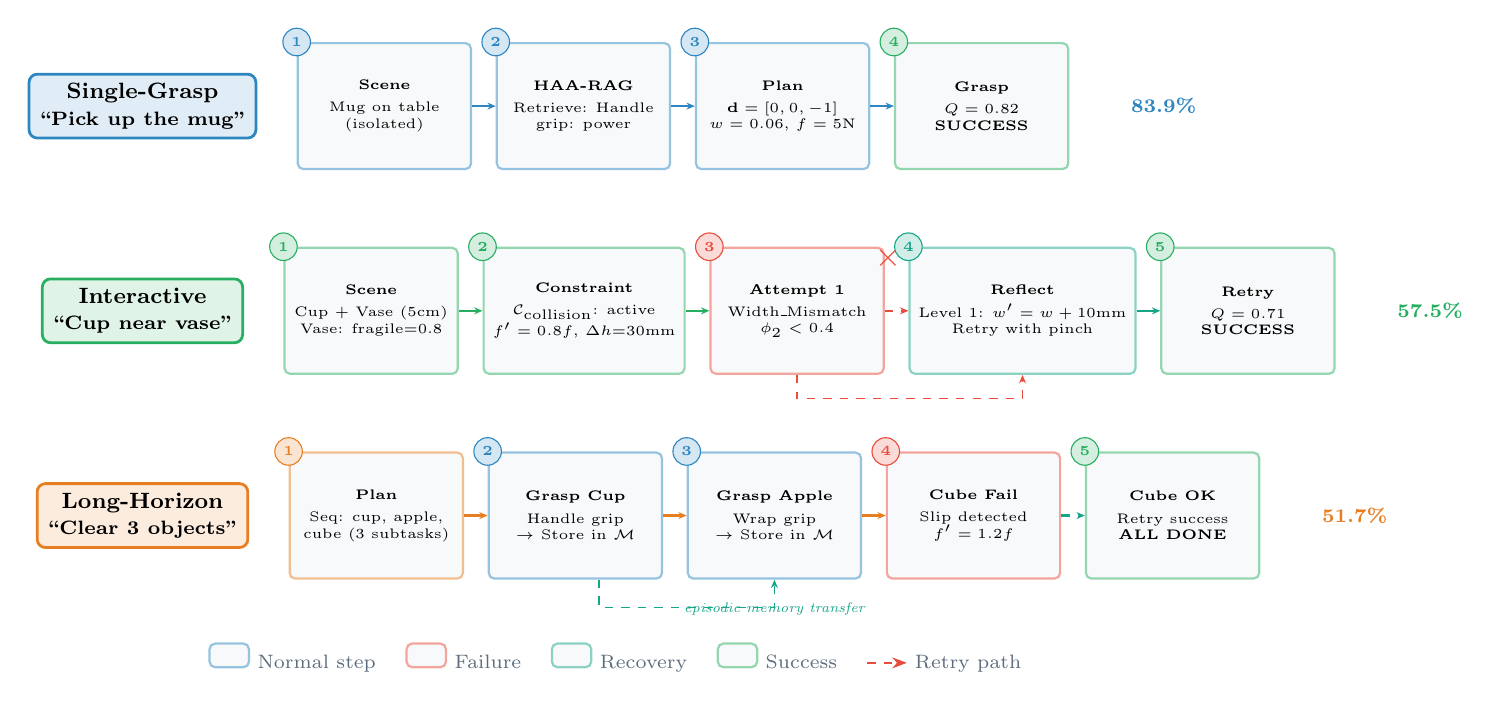
\begin{tikzpicture}[
  >=Stealth,
  node distance=0.3cm,
  frame/.style={
    rectangle, draw=#1!50, fill=framebg, line width=0.8pt,
    minimum width=2.2cm, minimum height=1.6cm,
    rounded corners=2pt, align=center, font=\tiny
  },
  steplabel/.style={
    circle, draw=#1, fill=#1!20, minimum size=0.35cm,
    font=\tiny\bfseries, text=#1, inner sep=0pt
  },
  tasklabel/.style={
    rectangle, rounded corners=3pt,
    draw=#1, fill=#1!15, line width=1pt,
    font=\footnotesize\bfseries, text=black, align=center,
    minimum height=0.5cm
  },
  myarrow/.style={
    ->, line width=0.8pt, color=#1,
    >={Stealth[length=3pt, width=2.5pt]}
  }
]

% ================================================================
% ROW 1: Single-Grasp Task (cup)
% ================================================================
\node[tasklabel=sgblue, minimum width=2.5cm] (sg_label) at (-5, 0) 
  {Single-Grasp\\{\scriptsize ``Pick up the mug''}};

% Frames
\node[frame=sgblue, right=0.5cm of sg_label] (sg1) {
  \textbf{Scene}\\[2pt]
  {\tiny Mug on table}\\
  {\tiny (isolated)}
};
\node[steplabel=sgblue] at (sg1.north west) {1};

\node[frame=sgblue, right=0.3cm of sg1] (sg2) {
  \textbf{HAA-RAG}\\[2pt]
  {\tiny Retrieve: Handle}\\
  {\tiny grip: power}
};
\node[steplabel=sgblue] at (sg2.north west) {2};

\node[frame=sgblue, right=0.3cm of sg2] (sg3) {
  \textbf{Plan}\\[2pt]
  {\tiny $\mathbf{d}=[0,0,-1]$}\\
  {\tiny $w=0.06$, $f=5$N}
};
\node[steplabel=sgblue] at (sg3.north west) {3};

\node[frame=successgreen, right=0.3cm of sg3] (sg4) {
  \textbf{Grasp}\\[2pt]
  {\tiny $Q = 0.82$}\\
  {\tiny \textbf{SUCCESS}}
};
\node[steplabel=successgreen] at (sg4.north west) {4};
\node[font=\Large, text=successgreen] at ($(sg4.east)+(0.3,0)$) {\checkmark};

% Arrows
\draw[myarrow=sgblue] (sg1) -- (sg2);
\draw[myarrow=sgblue] (sg2) -- (sg3);
\draw[myarrow=sgblue] (sg3) -- (sg4);

% ================================================================
% ROW 2: Interactive Task (cup near fragile vase) - with recovery
% ================================================================
\node[tasklabel=itgreen, minimum width=2.5cm] (it_label) at (-5, -2.6) 
  {Interactive\\{\scriptsize ``Cup near vase''}};

\node[frame=itgreen, right=0.5cm of it_label] (it1) {
  \textbf{Scene}\\[2pt]
  {\tiny Cup + Vase (5cm)}\\
  {\tiny Vase: fragile=0.8}
};
\node[steplabel=itgreen] at (it1.north west) {1};

\node[frame=itgreen, right=0.3cm of it1] (it2) {
  \textbf{Constraint}\\[2pt]
  {\tiny $\mathcal{C}_\text{collision}$: active}\\
  {\tiny $f'=0.8f$, $\Delta h$=30mm}
};
\node[steplabel=itgreen] at (it2.north west) {2};

\node[frame=failred, right=0.3cm of it2] (it3) {
  \textbf{Attempt 1}\\[2pt]
  {\tiny Width\_Mismatch}\\
  {\tiny $\phi_2 < 0.4$}
};
\node[steplabel=failred] at (it3.north west) {3};
\node[font=\large, text=failred] at ($(it3.north east)+(0.05,-0.15)$) {$\times$};

\node[frame=recoveryteal, right=0.3cm of it3] (it4) {
  \textbf{Reflect}\\[2pt]
  {\tiny Level 1: $w'=w+10$mm}\\
  {\tiny Retry with pinch}
};
\node[steplabel=recoveryteal] at (it4.north west) {4};

\node[frame=successgreen, right=0.3cm of it4] (it5) {
  \textbf{Retry}\\[2pt]
  {\tiny $Q = 0.71$}\\
  {\tiny \textbf{SUCCESS}}
};
\node[steplabel=successgreen] at (it5.north west) {5};
\node[font=\Large, text=successgreen] at ($(it5.east)+(0.3,0)$) {\checkmark};

\draw[myarrow=itgreen] (it1) -- (it2);
\draw[myarrow=itgreen] (it2) -- (it3);
\draw[myarrow=failred, dashed] (it3) -- (it4);
\draw[myarrow=recoveryteal] (it4) -- (it5);

% Recovery arc
\draw[myarrow=failred, dashed, line width=0.5pt] 
  (it3.south) -- ++(0, -0.3) -- ($(it4.south)+(0, -0.3)$) -- (it4.south);

% ================================================================
% ROW 3: Long-Horizon Task (clear table: 3 objects)
% ================================================================
\node[tasklabel=lhorange, minimum width=2.5cm] (lh_label) at (-5, -5.2)
  {Long-Horizon\\{\scriptsize ``Clear 3 objects''}};

\node[frame=lhorange, right=0.5cm of lh_label] (lh1) {
  \textbf{Plan}\\[2pt]
  {\tiny Seq: cup, apple,}\\
  {\tiny cube (3 subtasks)}
};
\node[steplabel=lhorange] at (lh1.north west) {1};

\node[frame=sgblue, right=0.3cm of lh1] (lh2) {
  \textbf{Grasp Cup}\\[2pt]
  {\tiny Handle grip}\\
  {\tiny $\to$ Store in $\mathcal{M}$}
};
\node[steplabel=sgblue] at (lh2.north west) {2};

\node[frame=sgblue, right=0.3cm of lh2] (lh3) {
  \textbf{Grasp Apple}\\[2pt]
  {\tiny Wrap grip}\\
  {\tiny $\to$ Store in $\mathcal{M}$}
};
\node[steplabel=sgblue] at (lh3.north west) {3};

\node[frame=failred, right=0.3cm of lh3] (lh4) {
  \textbf{Cube Fail}\\[2pt]
  {\tiny Slip detected}\\
  {\tiny $f' = 1.2f$}
};
\node[steplabel=failred] at (lh4.north west) {4};

\node[frame=successgreen, right=0.3cm of lh4] (lh5) {
  \textbf{Cube OK}\\[2pt]
  {\tiny Retry success}\\
  {\tiny \textbf{ALL DONE}}
};
\node[steplabel=successgreen] at (lh5.north west) {5};
\node[font=\Large, text=successgreen] at ($(lh5.east)+(0.3,0)$) {\checkmark};

\draw[myarrow=lhorange] (lh1) -- (lh2);
\draw[myarrow=lhorange] (lh2) -- (lh3);
\draw[myarrow=lhorange] (lh3) -- (lh4);
\draw[myarrow=recoveryteal, dashed] (lh4) -- (lh5);

% Memory transfer annotation
\draw[myarrow=recoveryteal, line width=0.5pt, dashed] 
  ($(lh2.south)+(0.3, 0)$) -- ++(0, -0.35) -- ($(lh3.south)+(0, -0.35)$) -- (lh3.south)
  node[midway, below, font=\tiny\itshape, text=recoveryteal] {episodic memory transfer};

% ================================================================
% LEGEND (bottom)
% ================================================================
\node[font=\scriptsize, text=textgray] at (1, -7) {
  \tikz{\node[frame=sgblue, minimum width=0.5cm, minimum height=0.3cm] {};} Normal step \quad
  \tikz{\node[frame=failred, minimum width=0.5cm, minimum height=0.3cm] {};} Failure \quad
  \tikz{\node[frame=recoveryteal, minimum width=0.5cm, minimum height=0.3cm] {};} Recovery \quad
  \tikz{\node[frame=successgreen, minimum width=0.5cm, minimum height=0.3cm] {};} Success \quad
  \tikz{\draw[->, dashed, failred, line width=0.5pt] (0,0) -- (0.5,0);} Retry path
};

% Category labels on right margin
\node[font=\scriptsize\bfseries, text=sgblue, rotate=0] at ($(sg4.east)+(1.2,0)$) {83.9\%};
\node[font=\scriptsize\bfseries, text=itgreen, rotate=0] at ($(it5.east)+(1.2,0)$) {57.5\%};
\node[font=\scriptsize\bfseries, text=lhorange, rotate=0] at ($(lh5.east)+(1.2,0)$) {51.7\%};

\end{tikzpicture}
\end{document}
